\documentclass[12pt,a4paper]{article}
\usepackage[utf8]{inputenc}
\usepackage[danish]{babel}
\usepackage{amsmath}
\usepackage{amsfonts}
\usepackage{amssymb}
\usepackage{graphicx}
\usepackage[left=2cm,right=2cm,top=2cm,bottom=2cm]{geometry}

%KEMI ORBITAL SRP%

\usepackage[x11names]{xcolor}
\usepackage{tcolorbox}% no need in this mwe
\usepackage[font=small]{caption}% no need in this mwe
\usepackage{float}% no need in this mwe
\usepackage{floatflt}% no need in this mwe

\usepackage{tikz} 
\usepackage{tikzorbital}
\usetikzlibrary{fadings,patterns,backgrounds,fit,arrows}
\pgfdeclarelayer{backbackground}
\pgfsetlayers{backbackground,background,main}

%%%%%%%%%%%%%%%%%%%%%%%%%%%%%%%%%%%%%%%%

\usepackage{titlepic}
\usepackage{enumerate}
\usepackage{enumitem}
\usepackage{float}
\usepackage{pdfpages}
\usepackage[colorlinks = true,
            linkcolor = blue,
            urlcolor  = blue,
            citecolor = blue,
            anchorcolor = blue]{hyperref}
\usepackage[explicit]{titlesec}
\usepackage{pstricks}
\usepackage[amsmath,thmmarks]{ntheorem} %pakke til at lave sætningsenvorinmets (kan ikke loades sammen med amsthm)
\usepackage{color}
\usepackage{tikz}

%opretter environmets til sætningsstrukturen 
\theorembodyfont{\normalfont}

	
	%sætnings environment	
	\newtheorem{thm}{Sætning}

	\theoremstyle{break}	
	%opgave environment	
	\newtheorem{opg}{Opgave}	

	%Korrolar environment
	\newtheorem{korollar}[thm]{Korollar}	
	
	%Lemma environment	
	\newtheorem{lemma}[thm]{Lemma}
	
	\theoremsymbol{\ensuremath{\circ}}	
	
	%definition environment	
	\newtheorem{definition}[thm]{Definition}
	
	%eksempel environment	
	\newtheorem{eksempel}[thm]{Eksempel}
	
	
	
	%Bevis environment
	\theoremstyle{nonumberplain}
	\theoremheaderfont{%
	\normalfont\itshape}
	\theorembodyfont{\normalfont}
	\theoremsymbol{\ensuremath{\square}}
	\theoremseparator{.}
	
	\newtheorem{proof}{Bevis}
	\newtheorem{los}{Løsning}
	

%% TEGNING TIL HOOKS LOV
\usetikzlibrary{decorations.pathmorphing,patterns}
%%




\setlength\parindent{0pt}

%\titleformat{\section}{\Large\bfseries}{}{0pt}{#1}
%\titleformat{\subsection}{\large\bfseries}{}{0pt}{#1}


%nye komandoer
\newcommand{\mR}{\mathbb{R}}
\newcommand{\mZ}{\mathbb{Z}}
\newcommand{\mN}{\mathbb{N}}
\newcommand{\mQ}{\mathbb{Q}}
\newcommand{\mC}{\mathbb{C}}
\newcommand{\hs}{\hspace{2mm}}
\newcommand{\Hs}{\hspace{4mm}}
\newcommand{\pipe}{\hs | \hs}
\newcommand{\lp}{\left(}
\newcommand{\rp}{\right)}
\newcommand{\vect}[1]{\underline{#1}}
\newcommand{\matr}[1]{\underline{\underline{#1}}}
\newcommand{\cnum}[1]{\raisebox{.5pt}{\textcircled{\raisebox{-.9pt} {#1}}}}




\author{Sebastian Borgund Hansen \\ 3r, Nørre Gymnasium}
\title{SRP - Kemi \& Fysik}
\date{\today}



\begin{document}
\maketitle
\section{Kovalente bindinger og organiske molekyler}

Mange kemiske forbindelser indeholder ikke ioner, men består i stedet af atomer, som er bundet tæt sammen i det vi kalder molekyler. Disse bånd, der holder atomerne sammen, formes når de omkredsende elektroner deles af de to kerner og derfor skaber noget stabilitet. Et sådan bånd kaldes et kovalent bånd. I modsætning til ion-bindinger dannes kovalente bindinger når ingen af de to atomkerner der indgår i bindingen har en stor nok elektronegativitet til at $rive$ elektronen væk fra det andet atom. Et af de simpleste eksempler på en kovalent binding er molekylet $H_2$. Kovalente bindinger er af stor betydning for den infrarøde-spektroskopi på grund af kovalente bindinger kan betragtes som fjedre som vi fra fysikkens verden kender meget til.

Vi vil se nærmere på dette i de følgende afsnit men først vil vi indledningsvist snakke om atomernes elektronkonfiguration. 


\subsection{Elektroner}
Fra fysikkens verden ved vi følgende ting om elektroner. 

\begin{enumerate}
\item En elektrons position kan ikke bestemmes nøjagtigt. Det vi til gengæld kan sige noget om, er den orbital som elektronen befinder sig i. Vi kan bestemme størrelsen og formen på den orbital hvor der er en relativt stor chance for at finde den enkelte elektron i.

\item De orbitaler som elektronerne bevæger sig i karakteriseres ved en kvantenumrene $n = 1,2,3 ...$. Når n bliver større bliver afstanden til kernen større. Tilsvarende bliver energierne for orbitalerne også større med et større n. For n større end 1 kan der godt være forskellige orbitaler, som har samme værdi for n. En elektronskal indeholder orbitaler med samme værdi for n. Vi kan derfor vælge at benævne skallerne ved deres kvantenumre $1,2,3,4,5,6,7$ eller respektivt med bogstaverne $K,L,M,N,O,P,Q$. 

\item Orbitaler, som har den samme værdi for n har nødvendigvis forskellige former. Her kan der referes til $2s$ og $2p$ orbitalerne, der behandles i afsnit 1.2.
\end{enumerate}

Det er desuden værd at noteres sig, at for et atom med mere end 2 elektroner


\subsection{Orbitaler}
For at forstå hvorfor to atomer vælger at gå sammen om at danne en binding hvori de deler deres elektroner er vi nødsaget til lige at betragte et enkelt atoms elektronkonfiguration. De subatomare entiteter som elektroner er opfører sig ikke lige så pænt som Bohr formulerede i hans atommodel, hvor elektronerne bevæger sig i cirkulære baner, eller skaller, rundt omkring atomets kerne. Ifølge nyere MOT (Læs: Molekylær Orbital Teori) har elektronerne en chance for at eksistere i visse områder omkring atomet. Disse områder er bestemt af hvor mange elektroner atomet har. Idéen om skallerne er ikke fuldstændig, men den molekylære orbital teori udbyggger de enkelte skaller, der behandles i Bohr model, med nogle undergrupper, som kaldes orbitaler. Det laveste energiniveau en elektron kan befinde sig i, når det bevæger sig rundt om atomkernen er kugleformet og har tildelt navnet 1s orbitalen. Figur 1 er en skitse af 1s orbitalen. 

\begin{figure}[ht!]
  \centering
  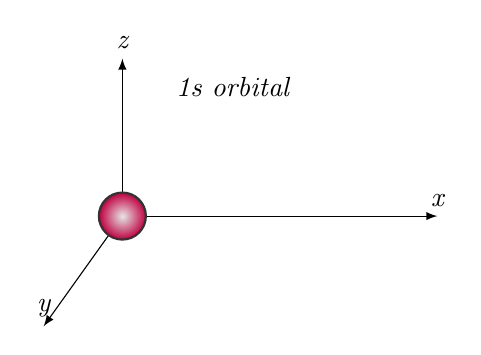
\begin{tikzpicture}[scale=2]
  \begin{scope}[font=\itshape]% to not type it every time, but better go for math mode


  \draw[-latex] (5,0)--(7,0) node[above]{x};
  \draw[-latex] (5,0)--(4.5,-0.7) node[above]{y};
  \draw[-latex] (5,0)--(5,1) node[above]{z};
  \orbital[color = purple, pos = {(5,0)}]{s} 
  \node[above] at (5.7,0.7) {1s orbital};

 		
  \end{scope}

  % correctly setting the background layer
  \begin{pgfonlayer}{backbackground}
  \fill[white](current bounding box.south west)rectangle
  (current bounding box.north east);
  \end{pgfonlayer}
  \end{tikzpicture}
  \caption{1s orbital} \end{figure}
  
  I s-orbitalerne er der plads til netop 2 elektroner. At den første orbital hedder 1s henviser til at den tilhører skal 1. I 2. skal tilhører elektronerne 2s orbitalen. s fordi at orbitalen er kugleformet og 2 fordi orbitalen knytter sig til 2. skal. Orbitalen ligner 1s orbitalen til forveksling, men vil have en større radius da elektronerne der befinder sig i denne orbital har mere energi. Da vi ved, at der skal være 8 elektroner i den 2. skal for, at oktetreglen er opfyldt og atomerne derfor er stabile mangler vi stadigvæk at placere 6 elektroner. Disse elektroner vil befinde sig i de såkaldte p-orbitaler. Der eksisterer 3 forskellige p-orbitaler, som ligner sløjfer og som hver især indeholder 2 elektroner. De tre p-orbitaler benævnes respektivt $p_x$, $p_y$ og $p_z$, da de er ortogonale på hinanden og ligger langs hhv. x, y og z aksen. De er på figur 2 illustreret i et kartesisk koordinatsystem.
  
TEST
 
\begin{figure}[ht!]
  \centering
  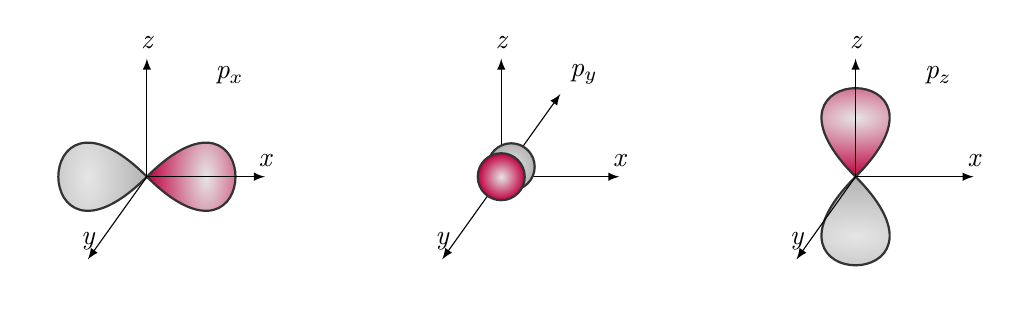
\begin{tikzpicture}[scale=1.5]
  \begin{scope}[font=\itshape]% to not type it every time, but better go for math mode

 \draw[-latex] (0,0)--(1,0) node[above]{x};
  \draw[-latex] (0,0)--(-0.5,-0.7) node[above]{y};
  \draw[-latex] (0,0)--(0,1) node[above]{z};
  \orbital[pcolor = purple, pos = {(0,0)}]{py}
  \node[above] at (0.7,0.7) {p$_x$};
	
  \draw[-latex] (3,0)--(3.5,0.7);
  \draw[-latex] (3,0)--(4,0) node[above]{x};
  \draw[-latex] (3,0)--(2.5,-0.7) node[above]{y};
  \draw[-latex] (3,0)--(3,1) node[above]{z};
  \orbital[pcolor = purple, pos = {(3,0)}]{px} 
  \node[above] at (3.7,0.7) {p$_y$};

  \draw[-latex] (6,0)--(7,0) node[above]{x};
  \draw[-latex] (6,0)--(5.5,-0.7) node[above]{y};
  \draw[-latex] (6,0)--(6,1) node[above]{z};
  \orbital[pcolor = purple, pos = {(6,0)}]{pz}
  \node[above] at (6.7,0.7) {p$_z$};
  \end{scope}
  % correctly setting the background layer
  \begin{pgfonlayer}{backbackground}
  \fill[white](current bounding box.south west)rectangle
  (current bounding box.north east);
  \end{pgfonlayer}
  \end{tikzpicture}
  \caption{$2p_x$, $2p_y$, $2p_z$ orbital} \end{figure}

I 3 skal kan der være 18 elektroner. Disse elektroner bliver først fyldt ind i en 3s orbital, der ligner både 1s og 2s orbitalen i og med, at den er kugleformet. Radius på 3s orbitalen er større end på 2s orbitalen grundet det højere energiniveau. 6 af de resterende 16 elektroner kan dernæst findes i 3p orbitalerne. Der er, ligesom 2p-orbitalerne, også tre 3p-orbitaler - $3p_x$,$3p_y$ og en $3p_z$ orbital. For det illustrative formål kan vi bare betragte 2p-orbitalerne. 3p-orbitalerne ligner dem, men elektronerne kan bare befinde sig i større sløjfer end 2p-orbitalerne. 

Nu har vi kigget på de simpleste af orbitalerne, s- og p-orbitalerne. Der eksisterer også d og f orbitaler. f-orbitalerne vil jeg ikke beskæftige mig med, men p-orbitalerne er illustretet  figur 3. (Se figur 3 og 4) 
\\

\begin{figure}[ht!]
  \centering
  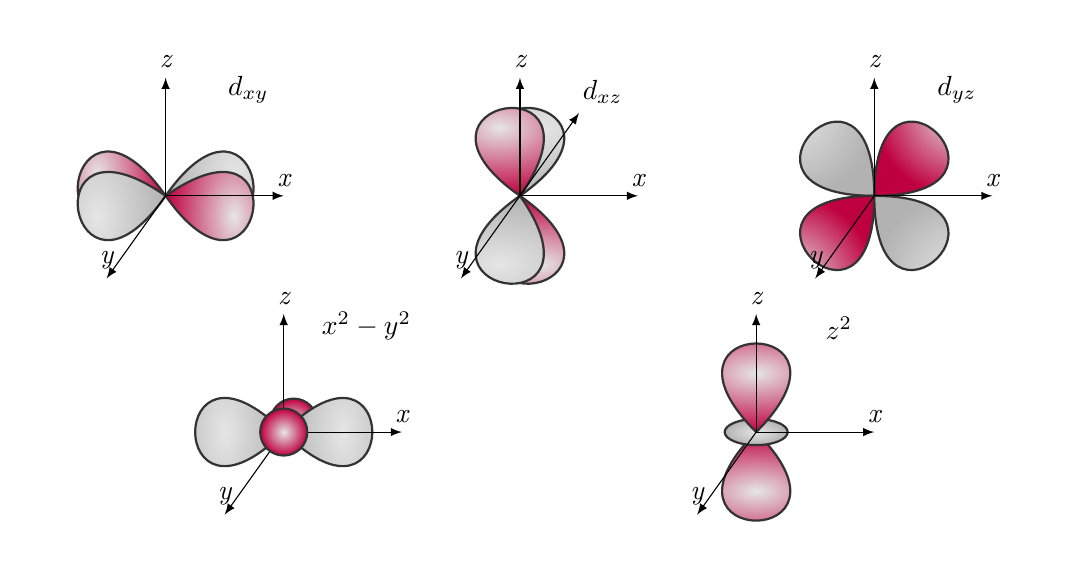
\begin{tikzpicture}[scale=1.5]
  \begin{scope}[font=\itshape]% to not type it every time, but better go for math mode

 \draw[-latex] (0,0)--(1,0) node[above]{x};
  \draw[-latex] (0,0)--(-0.5,-0.7) node[above]{y};
  \draw[-latex] (0,0)--(0,1) node[above]{z};
  \orbital[pcolor = purple, pos = {(0,0)}]{dxy}
  \node[above] at (0.7,0.7) {$d_{xy}$};
	
  \draw[-latex] (3,0)--(3.5,0.7);
  \draw[-latex] (3,0)--(4,0) node[above]{x};
  \draw[-latex] (3,0)--(2.5,-0.7) node[above]{y};
  \draw[-latex] (3,0)--(3,1) node[above]{z};
  \orbital[pcolor = purple, pos = {(3,0)}]{dxz} 
  \node[above] at (3.7,0.7) {$d_{xz}$};

  \draw[-latex] (6,0)--(7,0) node[above]{x};
  \draw[-latex] (6,0)--(5.5,-0.7) node[above]{y};
  \draw[-latex] (6,0)--(6,1) node[above]{z};
  \orbital[pcolor = purple, pos = {(6,0)}]{dyz}
  \node[above] at (6.7,0.7) {$d_{yz}$};
  
  \draw[-latex] (1,-2)--(2,-2) node[above]{x};
  \draw[-latex] (1,-2)--(0.5,-2.7) node[above]{y};
  \draw[-latex] (1,-2)--(1,-1) node[above]{z};
  \orbital[pcolor = purple, pos = {(1,-2)}]{dx2y2}
  \node[above] at (1.7,-1.3) {$x^{2}-y^{2}$};

  \draw[-latex] (5,-2)--(6,-2) node[above]{x};
  \draw[-latex] (5,-2)--(4.5,-2.7) node[above]{y};
  \draw[-latex] (5,-2)--(5,-1) node[above]{z};
  \orbital[pcolor = purple, pos = {(5,-2)}]{dz2}
  \node[above] at (5.7,-1.3) {$z^2$};
  
  \end{scope}
  % correctly setting the background layer
  \begin{pgfonlayer}{backbackground}
  \fill[white](current bounding box.south west)rectangle
  (current bounding box.north east);
  \end{pgfonlayer}
  \end{tikzpicture}
  \caption{$d_{xy}$, $d_{xz}$, $d_{yz}$, $x^{2}-y^{2}$, $z^2$ orbitalerne} 
  \end{figure}

\subsection{MO-teori}
I molekylær orbital teori, forkortet MO-teori, ses der på fordelingen af elektroner i molekyler på samme måde som vi ser på molekyler i atomer (FODNOTE TIL GENERAL CHEMISTRY s.149 mangler). Måden hvorpå vi bestemmer hvordan en elektron opfører sig på i et molekyle er ved hjælp af kvantemekanik og en bølgefunktion $\Psi$. På denne måde kan energien af en elektron og formen på det område hvori en elektron bevæger sig i bestemmes. Dette vil jeg kun berøre sporadisk. Som vi i afsnit 1.1 fandt ud af at elektroner i forskellige energiniveauer havde størst chance for at eksistere i forskellige områder som vi kaldte orbitaler, ligeså har elektroner i molekyler også orbitaler som de har en stor chance for at eksistere i. Forskellen er bare, at i molekyler kan elektronerne findes nær kernen på en hvilken som helst kerne, der indgår i molekylet; hvilket er hvorfor vi kalder disse orbitaler for molekylære elektronorbitaler eller bare molekylære orbitaler. 
Ligesom atomare orbitaler er molekyære orbitaler også fyldt når de indeholder præcist 2 orbitaler med modsat spin. 
\\

\subsubsection{$\pi$- \& $\sigma$-orbitaler}

Da vi så de atomare orbitaler gav vi dem navnene, s,p,d og f. Molekylære orbitaler har også navne, men jeg vil i denne opgave primært have fokus på hhv. $\pi$-orbitaler og $\sigma$-orbitaler. Vi betragter et eksempel med et homonukleært diatomisk molekyle som $H_2$. De to hydrogenatomer der er bundet sammen har hver deres egen elektron, men når de er sig tilpas tæt nok på hinanden vil elektronerne mere eller mindre befinde sig mellem de to kerner. Da elektronerne er negativt ladede og de 2 hydrogenkerner er positivt ladede, vil elektronerne blive tiltrukket af begge kerner og have et lavere niveau af energi end de ville have isolerede (MANGLER NOTE GENERAL CHEMISTRY SIDE 150). Da elektronerne søger at have en så lav energi som muligt vil de befinde sig mellem de to kerner og stabilisere molekylet. Denne slags orbitaler kaldes \textbf{bindende} orbitaler, da de som navnet antyder binder molekylet sammen. På figur 4 er det illustreret hvordan to atomare orbitaler går sammen om at danne en bindende $\sigma_s$ orbital. 
\begin{center}
\begin{figure}[ht!]
  \centering
  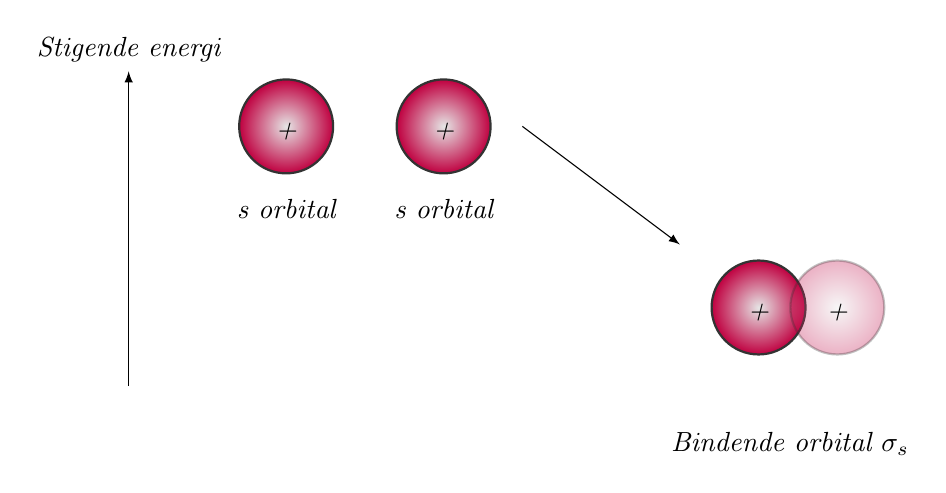
\begin{tikzpicture}[scale=2]
  \begin{scope}[font=\itshape]% 

  \draw[-latex] (0,-1)--(0,1) node[above]{Stigende energi};
  \orbital[color = purple, opacity = 1, scale = 2, pos = {(1,0.65)}]{s} 
  \orbital[color = purple, opacity = 1, scale = 2, pos = {(2,0.65)}]{s} 
  \node[above] at (1,0.5) {+};  
  \node[above] at (2,0.5) {+};
  \node[above] at (1,0) {s orbital};
  \node[above] at (2,0) {s orbital};
	\draw[-latex] (2.5,0.65)--(3.5,-0.10);
 		
 		
 		
 \orbital[color = purple, opacity = 1, scale = 2, pos = {(4,-0.5)}]{s} 
  \orbital[color = purple, opacity = 0.3, scale = 2, pos = {(4.5,-0.5)}]{s}  		
  \node[above] at (4.2,-1.5) {Bindende orbital $\sigma_s$};
 	\node[above] at (4,-0.65) {+}; 
 	\node[above] at (4.5,-0.65) {+}; 
  \end{scope}

  \begin{pgfonlayer}{backbackground}
  \fill[white](current bounding box.south west)rectangle
  (current bounding box.north east);
  \end{pgfonlayer}
  \end{tikzpicture}
  \caption{1s orbital} \end{figure}
	\end{center}
	
Denne bindende $\sigma$-orbital er faktisk det vi også kender som en $\sigma$-binding eller en kovalent binding. Kovalente bindinger er netop defineret som molekylære bindinger, der involverer at to atomer deler deres elektroner. 
\\

På samme måde som med $\sigma$-orbitalerne dannes $\pi$-orbitalerne ved, at to atomers befinder sig tæt på hinanden og elektronerne kan få en lavere energi ved at befinde sig i det sted hvor orbitalerne overlapper. $\pi$-orbitalerne adskiller sig alligevel fra $\sigma$-orbitalerne ved ikke at kunne blive dannet af overlap mellem s-orbitaler. En illustration af hvordan $\pi$-bindinger dannes ved et overlap af p-orbitaler: se figur 5. 

\begin{center}
\begin{figure}[ht!]
  \centering
  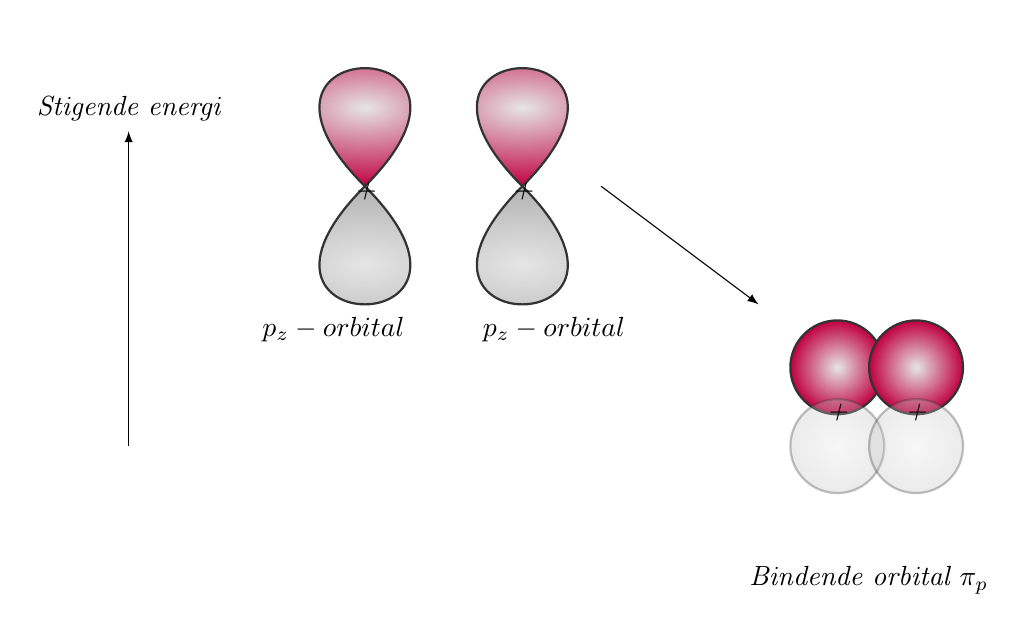
\begin{tikzpicture}[scale=2]
  \begin{scope}[font=\itshape]% 

  \draw[-latex] (-0.5,-1)--(-0.5,1) node[above]{Stigende energi};
  \orbital[pcolor = purple, opacity = 1, scale = 1, pos = {(1,0.65)}]{pz} 
  \orbital[pcolor = purple, opacity = 1, scale = 1, pos = {(2,0.65)}]{pz} 
  \node[above] at (0.8,-0.40) {$p_z-orbital$};
  \node[above] at (2.2,-0.40) {$p_z-orbital$};
	\draw[-latex] (2.5,0.65)--(3.5,-0.10);
  \node[above] at (1,0.5) {+};
  \node[above] at (2,0.5) {+};
 		
 \orbital[color = purple, opacity = 1, scale = 2, pos = {(4,-0.5)}]{s} 
  \orbital[color = purple, opacity = 1, scale = 2, pos = {(4.5,-0.5)}]{s}  	
  
 \orbital[color = lightgray, opacity = 0.3, scale = 2, pos = {(4,-1)}]{s} 
  \orbital[color = lightgray, opacity = 0.3, scale = 2, pos = {(4.5,-1)}]{s}  	  
  	
  \node[above] at (4.2,-2) {Bindende orbital $\pi_p$};
 		
 		
  \node[above] at (4,-0.90) {+};
  \node[above] at (4.5,-0.90) {+};		
 		
  \end{scope}

  \begin{pgfonlayer}{backbackground}
  \fill[white](current bounding box.south west)rectangle
  (current bounding box.north east);
  \end{pgfonlayer}
  \end{tikzpicture}
  \caption{1s orbital} \end{figure}
	\end{center}
\pagebreak
	
Nu har vi set på både $\sigma$-orbitaler /bindinger og $\pi$-orbitaler / bindinger - men hver for sig. Hvis de to orbitaler eksisterer sammentidigt i et molekyle har vi faktisk en dobbeltbinding. Dobbeltbindinger er netop en $\sigma$- og en $\pi$-binding. Illustret som en tegning ville det se ud på følgende måde, se Figur 6: 

\begin{center}
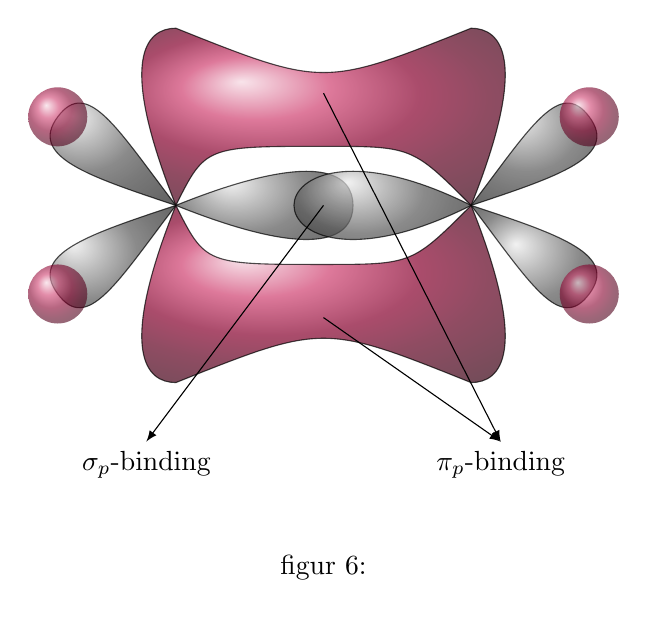
\begin{tikzpicture}[scale=0.75]

\shade[shading=ball, ball color=gray,draw,opacity=.7] (-2.5,0) .. controls (0,1) and     (.5,0.5) .. (.5,0)
.. controls (.5,-.5) and (0,-1) .. (-2.5,0);

\shade[shading=ball, ball color=gray,draw,opacity=.7] (2.5,0) .. controls (.5,1) and     (-.5,0.5) .. (-.5,0)
.. controls (-.5,-.5) and (.5,-1) .. (2.5,0);


\shade[shading=ball, ball color=gray,draw,opacity=.7] (-2.5,0) .. controls (-4,0.5) and     (-5,0.83) .. (-4.5,1.5)
.. controls (-4,2.17) and (-3.5,1.31) .. (-2.5,0);

\shade[shading=ball, ball color=gray,draw,opacity=.7] (-2.5,0) .. controls (-4,-0.5)     and (-5,-0.83) .. (-4.5,-1.5)
.. controls (-4,-2.17) and (-3.5,-1.31) .. (-2.5,0);


\shade[shading=ball, ball color=gray,draw,opacity=.7] (2.5,0) .. controls (4,0.5) and     (5,0.83) .. (4.5,1.5)
.. controls (4,2.17) and (3.5,1.31) .. (2.5,0);

\shade[shading=ball, ball color=gray,draw,opacity=.7] (2.5,0) .. controls (4,-0.5) and     (5,-0.83) .. (4.5,-1.5)
.. controls (4,-2.17) and (3.5,-1.31) .. (2.5,0);

\shade[shading=ball, ball color=purple,opacity=0.6] (4.5,1.5) circle (0.5);

\shade[shading=ball, ball color=purple,opacity=0.6] (4.5,-1.5) circle (.5);

\shade[shading=ball, ball color=purple,opacity=0.6] (-4.5,-1.5) circle (.5);

\shade[shading=ball, ball color=purple,opacity=0.6] (-4.5,1.5) circle (.5);


\shade[shading=ball, ball color=purple,draw,opacity=.7] (-2.5,0) .. controls (-3.5,2.5)     and (-3,3) .. (-2.5,3)
.. controls (0,2) .. (2.5,3)
.. controls (3,3) and (3.5,2.5) .. (2.5,0)
.. controls (1.5,1) .. (0,1)
.. controls (-2,1) .. (-2.5,0);


\shade[shading=ball, ball color=purple,draw,opacity=.7] (-2.5,0) .. controls (-3.5,-2.5)     and (-3,-3) .. (-2.5,-3)
.. controls (0,-2) .. (2.5,-3)
.. controls (3,-3) and (3.5,-2.5) .. (2.5,-0)
.. controls (1.5,-1) .. (0,-1)
.. controls (-2,-1) .. (-2.5,-0);

\draw[-latex] (0,0)--(-3,-4) node[below]{$\sigma_p$-binding};

\draw[-latex] (0,1.9)--(3,-4) node[below]{$\pi_p$-binding};

\draw[-latex] (0,-1.9)--(3,-4) node[below]{ };


\node[above] at (0,-6.5){figur 6: };
\end{tikzpicture}
\end{center}

$\sigma$-bindingerne er de stærkestee af de kovalente bindinger. Dernæst kommer $\pi$-bindingerne. blabla MO teori...


Det er nemmelig ikke alle atomer, der har mulighed for at danne kovalente bindinger imellem sig. Når 2 atomer går sammen om at danne en kovalent binding er det fordi, at de hver især er ustabile. At de er ustabile er ens betydende med, at de ikke har deres orbitaler af højeste energiniveau fyldt ud. Hver orbital vil gerne have en spin-op og en spin-ned elektron. Når nogle atomer så alligevel ikke vælger at gå sammen og danne en kovalent binding er det enten fordi, at de har for mange mange elektroner til, at de kun kan befinde sig mellem atomerne og danne en bindende $\sigma$-binding og derfor befinder sig i en orbital, der kræver et højere energiniveau og derfor er anti-bindende. 

\subsection{kovalente bindinger}
Så det vi fandt ud af i dette afsnit var, at når 2 atomer går sammen og deler deres elektroner for at opnå en lavere energitilstand dannes nogle bindinger som vi kalder kovalente bindinger. Kovalente bindinger dannes når atomer, der har lige stor tilbøjelighed til at afgive elektroner mødes. Et eksempel på et organisk molekyle, der dannes kovalente bindinger er ethylen. Her ses det tydeligt hvordan de to p-orbitaler går sammen i midten af molekylet om at lave en $\sigma_p$-(se figur 6). Delte elektroner findes primært mellem de positivt ladede atomkerner og den elektrostatiske tiltrækning mellem de to positivt ladede kerner og de to negativt ladede elektroner holder molekylet sammen. Det bånd der bliver dannet som et resultat af førnævnte er meget stærkt.

\section{IR-Spektroskopi}

\subsection{Fysikken bag}

\subsubsection{Arbejde og Hookes lov}
I den daglige omtale er arbejde et fysisk aktivitet der kræver energi. I fysikken bruger vi derimod arbejde som et udtryk for en kraft der virker på en genstand over en given distance. Arbejdet, A, som en genstand er blevet tilført på en strækning, s, med en kraft, F, er givet ved formlen
\\
\begin{center}
 $A=F \cdot s$. 
\end{center}
\bigskip

Dette er dog under antagelse af at kraften der virker på objektet er konstant samt at flytningen af objektet er i samme retning som kraften virker. 
Vi støder dog ind i problemer med at bestemme energien ud fra denne formel, hvis vi ser på et system hvor kraften bliver større jo længere væk fra startstedet, $s_0$, objektet bevæger sig. Formod nu, at vi ser på et objekt der bevæger sig langs en ret linje og hvor kraften bliver større jo længere vi flytter objektet. Da vil det samlede arbejde, $\sum A$ være lig summmen af alle de kræfter der har virket på objektet, siden størrelsen \textbf{arbejde} er en skalar.
\\
\begin{center}
$\sum A = A_1 + A_2 + ... + A_{n-1} + A_n$
\end{center}
\bigskip

For at bestemme denne størrelse deler vi den afstand, $s$, som objektet bevæger sig op i mindre dele $\Delta x_1$, $\Delta x_2$ osv. Vi deler disse afstande op i tilstrækkeligt små længder sådan at kraften der virker over de enkelte afstande er omtrent konstant. På denne måde kan vi beregne et totale arbejde som:
\\
\begin{center}
$A = F_1 \cdot \Delta x_1 + F_2 \cdot \Delta x_2 + ..$
\end{center}
\bigskip

Når vi får tilstrækkeligt mange længder og længderne samtidigt går mod at blive uendeligt små vil denne størrelse gå mod at blive integralet af F fra $x_1$ til $x_2$: 

\begin{center}
$A = \int\limits_{x_1}^{x_2} F dx$ 
\end{center}
\bigskip

Det er netop dette princip som Hookes lov benytter sig af. Hookes lov siger, at for en perfekt fjeder vil kraften direkte proportional til afstanden som fjederen er udtrukket. 

\begin{center}
$F = kx$
\end{center}
\bigskip

hvor k er stivheden er fjederen, F er kraften og x er den længden som fjederen er trukket ud. Med en perfekt fjeder skal der forstås at denne formel gælder uanset hvor langt man strækker fjederen ud eller presser den sammen. Dette er naturligvis en grov antagelse, men det er en god fysisk beskrivelse for at beregne størrelsen af en fjederkraft. Vi vil nu se på udledningen af denne sammenhæng.

Der vil her blive taget udgangspunkt i formlen 
\begin{equation}
V=\dfrac{1}{2} \cdot k \cdot (r-r_{0})^2
\end{equation}

Hvor V beskriver den potentielle energi en fjeder har når den er strukket en distance r ud fra hvilelængden $r_0$. 

\subsubsection{Udledning af Hookes lov}
Betragt den potentielle energi af en fjeder givet ved

\bigskip

\begin{equation}
V=\dfrac{1}{2} \cdot k \cdot (r-r_{0})^2
\end{equation}

\bigskip

Sæt nu $r_0 = 0$ og lad den initiale længde $r_i = r$ og den endelige udstrækningslængde $r_e = r + \Delta r$. Hvis vi ser på ændringen i den potentielle energi for systemet får vi da:

\bigskip

\begin{equation}
\Delta V = V_e - V_i = \dfrac{1}{2} \cdot k \cdot (r+ \Delta r)^2 - \dfrac{1}{2} \cdot k \cdot r^2
\end{equation}

\bigskip

Vi skriver $(r + \Delta r)^2$ ud og får:

\bigskip

\begin{equation}
\Delta V = V_e - V_i = \dfrac{1}{2} \cdot k \cdot (r^2 + 2r \Delta r + \Delta r^2) - \dfrac{1}{2} \cdot k \cdot r^2 
\end{equation}

\bigskip

I ligningen betragter vi nu de to størrelser $\dfrac{1}{2} \dot k \cdot r^2 og - \dfrac{1}{2} \cdot k \cdot r^2$. Disse to størrelser går ud med hinanden og efterlader os med

\bigskip

\begin{equation}
\Delta V = kr \Delta r + \dfrac{1}{2} \cdot k \cdot \Delta r^2
\end{equation}

\pagebreak
Vi noterer os nu, at det første led på højresiden af lighedstegnet er lineært i $\Delta r$ og at det andet led på højresiden af lighedstegnet er kvadreret i $\Delta r$. $\Delta r$ er en infinitesimal i kalkulus, hvilket betyder at størrelsen $\Delta r$ er meget mindre end 1. Når man så vælger at kvadrere noget der er strengt mindre end 1 og $\Delta r$ er så lille som muligt, hvilket er naturligt i kalkulusregning, går størrelsen $\dfrac{1}{2} \cdot k \cdot \Delta r^2$ mod 0. Så vi ender med

\bigskip

\begin{equation}
\Delta V = kr \Delta r
\end{equation} 

\bigskip

Dette udtryk beskriver altså ændringen i den potentielle energi når vi udstrækker fjederen $\Delta r$, der er en meget lille størrelse. 

\bigskip

Vi ser nu på ændringen for energi i et system, der er givet ved formlen 
\begin{equation}
\Delta E = \Delta E_kin + \Delta E_pot
\end{equation}

\bigskip

Ændringen i energi for et system er lig summen af ændringen i potentiel energi og kinetisk energi. 

Dette skulle meget gerne være lig 0 og vi får da 

\bigskip

\begin{equation}
\Delta E = \Delta E_{kin} + \Delta V = 0
\end{equation}

\bigskip

Hvilket, hvis størrelsen for den potentielle energi givet ved $\Delta V = kr \Delta r$ substitueres ind i stedet for $V$ i ligning  giver

\bigskip

\begin{equation}
\Delta E_{kin} + kr \Delta r = 0 \rightarrow \Delta E_kin = -kr \Delta r
\end{equation}

\bigskip

Nu vil vi bruge det fysiske resultat

\bigskip

\begin{equation}
\Delta E_{kin} = A = \textbf{F} \times \Delta \textbf{r} = F \cdot \Delta r (Arbejde-Energi teoremet)
\end{equation}

\bigskip

Notér at der i dette tilfælde regnes på en fjeder og der da kan ses bort fra at $F$ og $\Delta r$ begge normalt er vektorer og arbejdet da skal beregnes som krydsproduktet af de to vektorer da fjederen udstrækkes i samme retning som fjederen trækkes. Vi tillader os da at regne arbejdet som $F \cdot \Delta r = A$.

Nu bruger vi resultatet 

\bigskip

\begin{equation}
\Delta E_{pot} = \textbf{F} \times \Delta \textbf{r} = F \cdot \Delta \textbf{r} = -kr \Delta r
\end{equation}

\bigskip

Ved division på begge sider af lighedstegnet af ligningen 

\bigskip

\begin{equation}
F \cdot \Delta r = -kr \Delta r
\end{equation}

\bigskip

Får vi det ønskede resultat: 

\bigskip

\begin{equation}
F = -k \cdot r
\end{equation}

\bigskip

\subsubsection{Harmoniske svingninger}
En oscillerende bevægelse er en bevægelse hvor et objekt, som bliver flyttet fra sit hvilested og sluppet vil bevæge sig tilbage mod sit hvilested, hvor det vil bevæge sig forbi sit hvilested for igen at foretage gentagelser af netop dette for til slut at ende på sit hvilested igen. Dette kan eksempelvis ses hos penduler og masser bundet til fjedre.
\\

Eksemplet der vil blive betragtet i dette kapitel er oscillerende bevægelse, der er hensigtsmæssig i forhold til at forstå IR-spektroskopier. Vi vil se på en masse der er bundet til en fjeder. Se figur 7.

\begin{center}
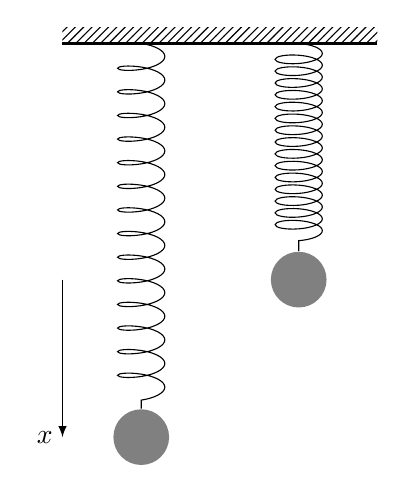
\begin{tikzpicture}
\node[circle,fill=gray,inner sep=2.5mm] (a) at (0,0) {};
\node[circle,fill=gray,inner sep=2.5mm] (b) at (2,2) {};
\draw[decoration={aspect=0.3, segment length=3mm, amplitude=3mm,coil},decorate] (0,5) -- (a); 
\draw[decoration={aspect=0.3, segment length=1.5mm, amplitude=3mm,coil},decorate] (2,5) -- (b); 
\fill [pattern = north east lines] (-1,5) rectangle (3,5.2);
\draw[thick] (-1,5) -- (3,5);

\draw[-latex] (-1,2)--(-1,0) node[left]{$x$};

\end{tikzpicture}
\end{center}

Med udgangspunkt i figur 7 vil vi se på en masse der i den ene ende er fastgjort til noget stationært og i den anden ende er fastgjort til en kugle med en masse. Når kuglen ikke påvirkes af andre ydre kræfter en tyngdekraften vil kuglen opnå en hviletilstand hvor fjederkraften er lige så stor som tyngdekraften. Vi sætter denne hviletilstand til $x_0=0$. Når vi så begynder at påvirke system med en ydre kraft ved f.eks. at hive i kuglen vil fjederen svare tilbage ved at trække endnu hårdere i kuglen. Hvis vi op som den positive retning vil vi på figur 7 have flyttet kuglen en afstand $-x$ væk fra sin hvileposition vil fjederkraften givet ved Hookes lov, der blev beskrevet i 2.1.2 være givet ved $F_x=-k \cdot x$. Hvor F er fjedekraften, k er fjederkonstanten for den givne fjeder og x er afstanden flyttet fra hvilepositionen $x_0$
\\

\subsubsection{Udledning af frekvens og positionsfunktion for harmonisk bevægelse}

Antag nu at Hookes lov gælder og at bevægelsen udelukkende foregår i y-aksens retning. Newton II giver da 

\bigskip

\begin{center}
$F_x = -k \cdot x = m \cdot a_x = m \cdot x'' \rightarrow a_x = -\dfrac{k}{m} \cdot x$
\end{center}

\bigskip

Hvis massen, m, af objektet der er fæstnet til fjederen er konstant er størrelsen $\dfrac{k}{m}$ bare en konstant og da er $a_x \propto x$ til et hvert tidspunkt. Ud fra dette kan vi se at accelerationen er størst når x har opnået sin højeste positive værdi, kald denne størrelse $x_{max}$. Ydermere vil accelerationen være lig 0 når objketet passerer sit hvilepunkt, da x er lig 0 i det punkt.
\pagebreak

Der bruges nu princippet om energibevarelse med den potentielle energi af systemet givet ved $V=\dfrac{1}{2} \cdot k \cdot x^2$, ligesom i afsnit 2.1.2 om Hookes lov, og den kinetiske energi af systemet givet ved $E_kin = \dfrac{1}{2} \cdot m \cdot v^2$.

\bigskip

\begin{center}
$E_{system}=\dfrac{1}{2} \cdot m \cdot v^2 + \dfrac{1}{2} \cdot k \cdot x^2 = konstant$
\end{center}

\begin{figure}[ht!]
  \centering
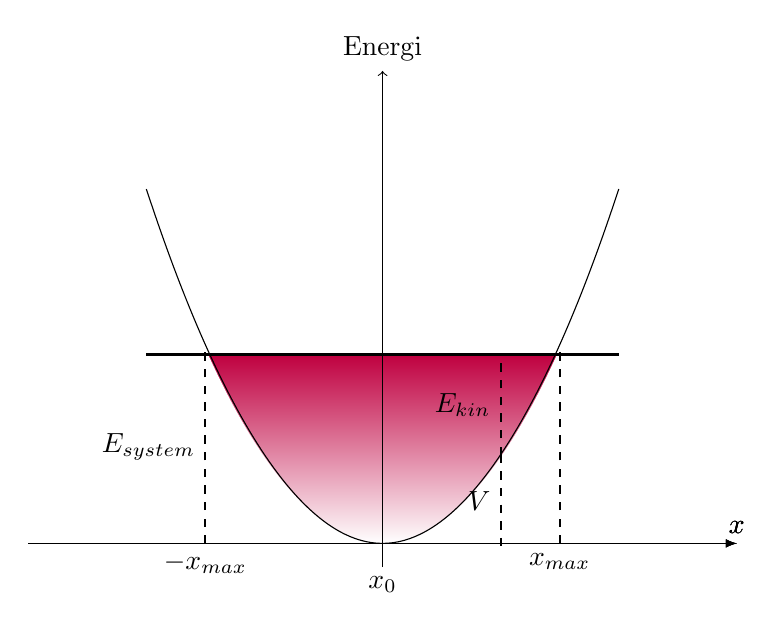
\begin{tikzpicture}[scale=1.5]
\shade[top color=purple,bottom color=white] (-1.49,0) rectangle (1.49,1.6);

\shade[top color=white,bottom color=white!50] 
      (0,0) parabola (1.5,1.65) |- (0,0);
\shade[top color=white,bottom color=white!50] 
      (0,0) parabola (-1.5,1.65) |- (0,0);      

  \draw[-latex] (-3,0) -- (3,0) node[above] {$x$};
  \draw[->] (0,-0.2) -- (0,4) node[above] {Energi};

  \draw (0,0) parabola bend (0,0) (2,3) node[below right] { };
  
  \draw (0,0) parabola bend (0,0) (-2,3) node[below right] { };
  
  \node[above] at (0,-0.5) {$x_0$};
  \draw[-latex] (-3,0) -- (3,0) node[above] {$x$};
	\draw[thick, dashed] (1,0.75) -- (1,1.6) node [midway, left] {$E_{kin}$};
	
	\draw[-latex] (-3,0) -- (3,0) node[above] {$x$};
	\draw[thick, dashed] (1,0.75) -- (1,-0.03) node [midway, left] {$V$};
	
	\draw[thick, dashed] (-1.5,0) -- (-1.5,1.63) node [midway, left] {$E_{system}$};
	
	\node[below] at (-1.5,0) {$-x_{max}$};
	
\draw[thick, dashed] (1.5,0) -- (1.5,1.63) node [midway, left] { };	

\node[below] at (1.5,0) {$x_{max}$};

\draw[very thick] (-2,1.6) -- (2,1.6) node [midway, left] { };

\end{tikzpicture}
\caption{$E_{system} $ for oscilerende bevægelse} \end{figure}

\bigskip

Den totale energi $E_{system}$ er ydermere også relateret til amplituden af $x_{max}$ sådan at når objektet når sin maksimale flytning $\pm x_{max}$ vil objektet stoppe og vende om. I dette punkt hastigheden $v = 0$ og objektet har altså ikke nogen kinetisk energi. I dette punkt er $E_{system } = \dfrac{1}{2} \cdot k \cdot x^2$. Derfor må det gælde at

\bigskip
\begin{center}
$E_{system}=\dfrac{1}{2} \cdot m \cdot v^2 + \dfrac{1}{2} \cdot k \cdot x^2 = \dfrac{1}{2} \cdot k \cdot (x_{max})^2$
\end{center}
\bigskip

eller 

\bigskip
\begin{center}
$\dfrac{1}{2} \cdot m \cdot v^2 + \dfrac{1}{2} \cdot k \cdot x^2 = \dfrac{1}{2} \cdot k \cdot (x_{max})^2 \rightarrow m \cdot v^2 = k \cdot (x_{max})^2 - k \cdot x^2 = k \cdot ((x_{max})^2 - x^2)$

$\rightarrow v^2 = \dfrac{k}{m} \cdot ((x_{max})^2 - x^2) \rightarrow v = \pm \sqrt[2]{\dfrac{k}{m}} \cdot \sqrt[2]{(x_{max})^2-x^2}$
\end{center}
\bigskip

Med forbehold for fortegnet kan vi bruge denne relation til at bestemme hastigheden af objektet til en hver position x. Vigtigheden af det fundne udtryk $v = \pm \sqrt[2]{\dfrac{k}{m}} \cdot \sqrt[2]{(x_{max})^2-x^2}$ gør sig tydligt på Figur (MANGLER) hvor energien er plottet op ad 2. aksen og udstrækningen fra hvilepositionen $x_0$ ad 1. aksen. Kurven repræsenterer den potentielle energi givet ved forskriften $V=\dfrac{1}{2} \cdot k \dot x^2$ og dette er en parabel. I højden E er der en tyk sort streg, som repræsenterer den energibevarelse der er for systemet, da den skærer parablen i netop $-x_{max}$ og $x_{max}$ som er yderpositionerne for bevægelsen. Til en vilkårlig udstrækning af fjederen kan vi også bestemme den kinetiske energi som længden af den linje, der går fra den horisontale linje ned til parablen ved netop den x-værdi. Dér hvor den kinetiske energi er størst og altså farten er størst er ved hvilepositionen $x_0$. Det gælder altså at

\bigskip
\begin{center}
$\dfrac{1}{2} \cdot m \cdot (v_{max})^2 = E_{system}$ eller $v_{max} = \sqrt[2]{\dfrac{2 \cdot E_{system}}{m}}$
\end{center}
\bigskip

Men da det netop gjorde sig gældende at den maksimale potentielle og kinetiske energi begge er lig systemets energi $E_{system}$, og derfor også til hinanden, kan vi relatere $v_{max}$ til $x_{max}$.

\begin{center}
\begin{equation}
E_{system} = \dfrac{1}{2} \cdot k \cdot (x_{max})^2 = \dfrac{1}{2} \cdot m \cdot (v_{max})^2 \rightarrow v_{max} = \sqrt[2]{\dfrac{k}{m}} \cdot x_{max}
\end{equation}
\end{center}

I ligning (MANGLER) fandt vi udtrykket $v = \pm \sqrt[2]{\dfrac{k}{m}} \cdot \sqrt[2]{(x_{max})^2-x^2}$. Dette beskrev hastigheden til en udstrækning x. Vi ser os ikke tilfredse med en hastighedsfunktion. Vi vil også have stedsfunktionen. Denne findes ved at skrive den fundne ligning op som 

\begin{center}
\begin{equation}
\dfrac{dx}{dt} = v = \pm \sqrt[2]{\dfrac{k}{m}} \cdot \sqrt[2]{(x_{max})^2-x^2}
\end{equation}
\end{center}

Men da kan ligningen integreres og løses for x, hvilket giver

\begin{center}
\begin{equation}
x = x_{max} \cdot sin(\sqrt[2]{\dfrac{k}{m}} \cdot t + C)
\end{equation}
\end{center}
\bigskip
Hvor C er en konstant. Notér at sinus er en periodisk funktion og at positionen af x altså også er en periodisk funktion af tiden, som vi forventede. Perioden for bevægelsen, T, er den tid det tager for systemet at lave en oscilation. Da sinusfunktionen gentager sig selv, hver eneste gang vi øger udtrykket inden i parantesen $sin(\sqrt[2]{\dfrac{k}{m}} \cdot t + C$ må det altså gælde, hvis vi starten til t = 0 at en oscilation må tage

\begin{center}
\begin{equation}
\sqrt[2]{\dfrac{k}{m}} \cdot T = 2 \pi \rightarrow T = 2 \pi \sqrt[2]{\dfrac{m}{k}}
\end{equation}
\end{center}

Hvilket hvis $f = \dfrac{1}{T}$ giver

\begin{center}
\begin{equation}
f = \dfrac{1}{T} = \dfrac{1}{2 \pi} \cdot \sqrt[2]{\dfrac{k}{m}}
\end{equation}
\end{center}

Hvilket er et vigtigt resultat, som vi vil bruge til at bestemme bølgetal for funktionelle grupper i IR-spektroskopien. 
\pagebreak
\subsection{Den bagvedlæggende kemi}

\end{document}